
%--------------------------------------------------------------------
\section{Blob-Based Motion Analysis}
%--------------------------------------------------------------------

\begin{frame}
    \frametitle{Blob-Based Motion Analysis}
    \framesubtitle{Methodology}

    \begin{enumerate}
        \item {\bf Global motion detection} using simple frame-by-frame 
            subtraction 
        \item {\bf Blob extraction} using Poppe et al.'s (2007) background 
            modeling method 
        \item {\bf Appearance-based blob tracking} using the 
            forward-backward overlap technique and the color coherence 
            vector (CCV) for occlusion handling 
        \item {\bf Blob feature vector discretization} using the $k$-means 
            algorithm
    \end{enumerate}

\end{frame}

%--------------------------------------------------------------------

\begin{frame}
    \frametitle{Blob-Based Motion Analysis}
    \framesubtitle{Methodology (cont.)}

    Preliminary report on the results for this {\bf appearance-based blob 
    tracking method} appeared in Gharti (2010)'s work. 
    
    \bigskip
    
    I worked with Gharti to produce the initial version of the method. 
    Since the initial implementation was simplistic in some cases and 
    some work was redundant, I improved the code to get better blob matching. 
    
    \bigskip
    
    In particular, the current implementation does not need to create and 
    label each group of merged tracks but use only the information gained 
    from the merged track association matrix. I also eliminated unnecessary 
    cases in the blob-to-track association process.

\end{frame}

%--------------------------------------------------------------------

\begin{frame}
    \frametitle{Blob-Based Motion Analysis}
    \framesubtitle{Sample Blob Tracking Results}

    \begin{figure}
        \centering
        \begin{tabular}{ccccc}
            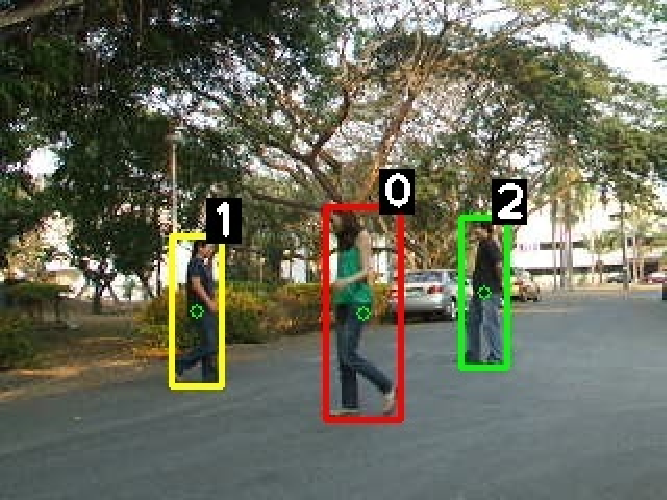
\includegraphics[scale=0.17]{figures/normal-tracking-result-0090} &
            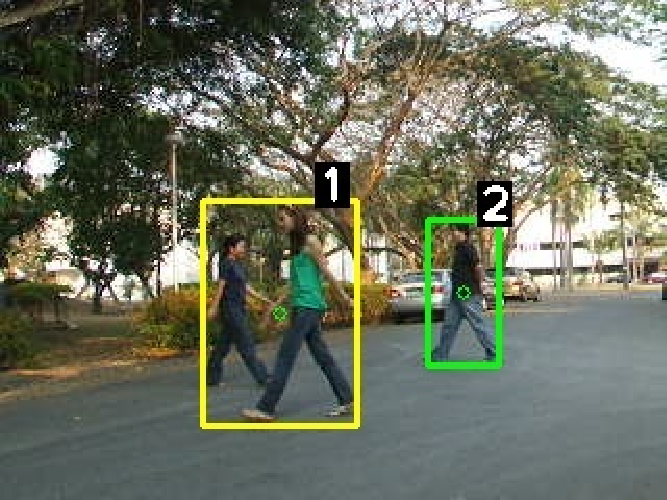
\includegraphics[scale=0.17]{figures/normal-tracking-result-0094} &
            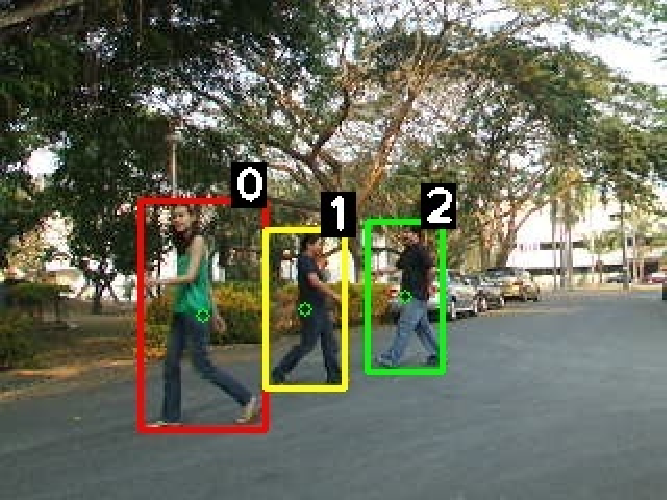
\includegraphics[scale=0.17]{figures/normal-tracking-result-0103} &
            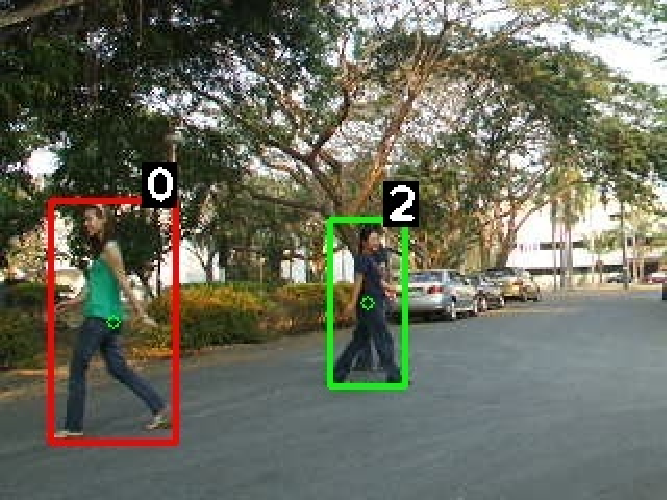
\includegraphics[scale=0.17]{figures/normal-tracking-result-0110} &
            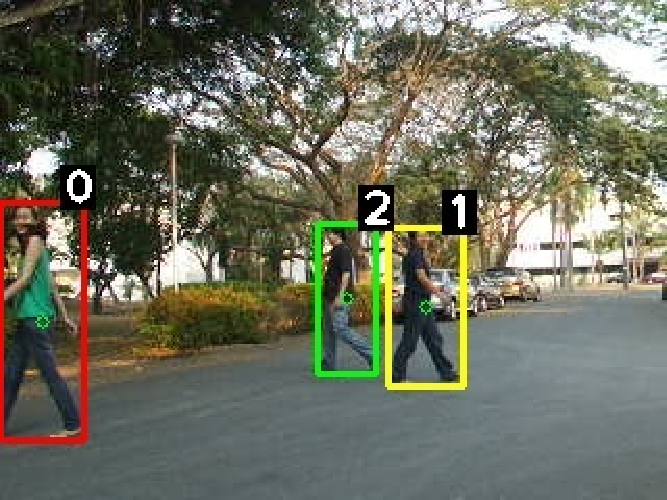
\includegraphics[scale=0.17]{figures/normal-tracking-result-0116} 
            \\
            \small Frame 90 & 
            \small Frame 94 & 
            \small Frame 103 & 
            \small Frame 110 & 
            \small Frame 116
        \end{tabular}
        \caption{Sample blob tracking results for typical simple
            cases.}
        \label{fig:normal-tracking-results}
    \end{figure}

    \begin{figure}
        \centering
        \begin{tabular}{ccccc}
            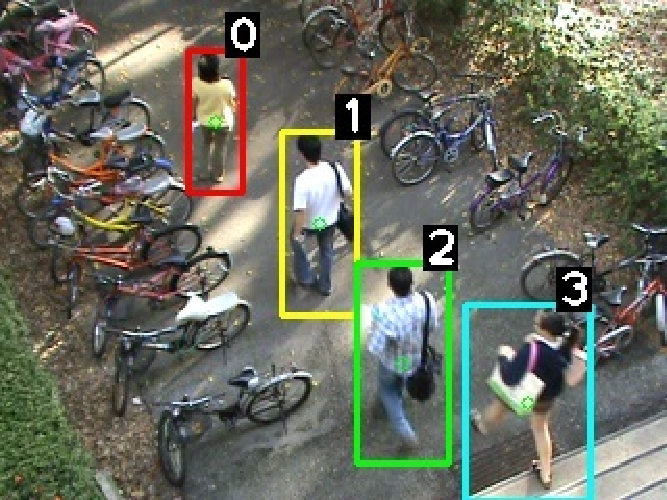
\includegraphics[scale=0.17]{figures/complex-tracking-result-0125} &
            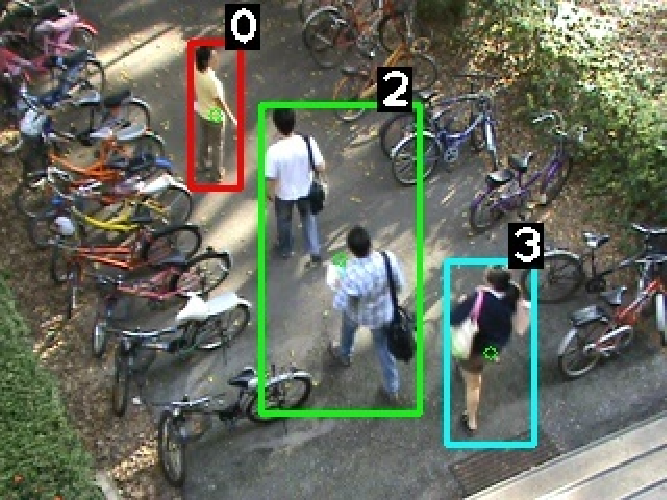
\includegraphics[scale=0.17]{figures/complex-tracking-result-0131} &
            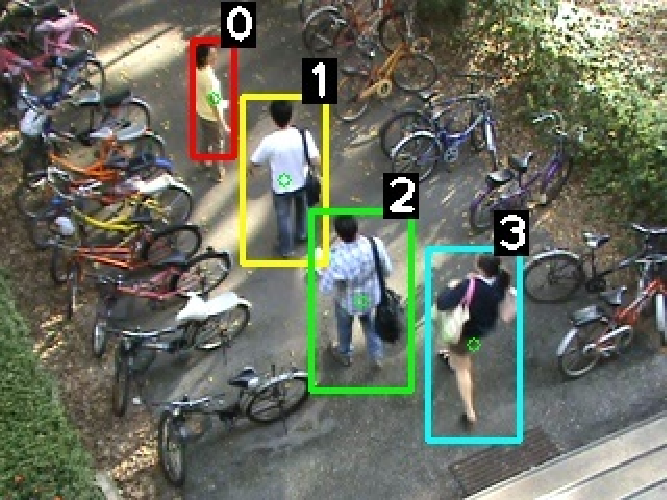
\includegraphics[scale=0.17]{figures/complex-tracking-result-0133} &
            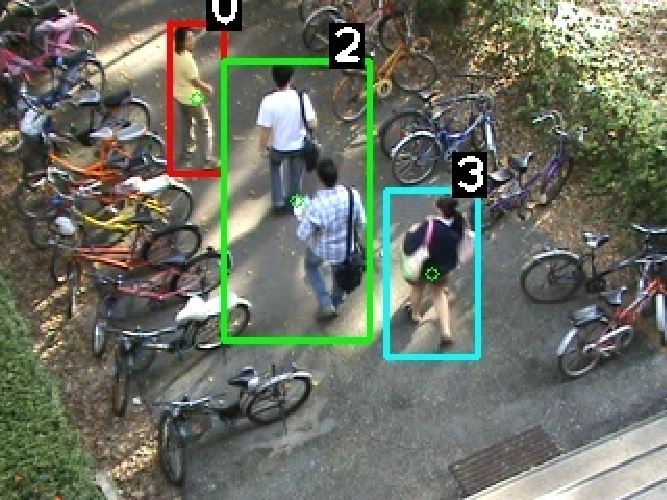
\includegraphics[scale=0.17]{figures/complex-tracking-result-0141} &
            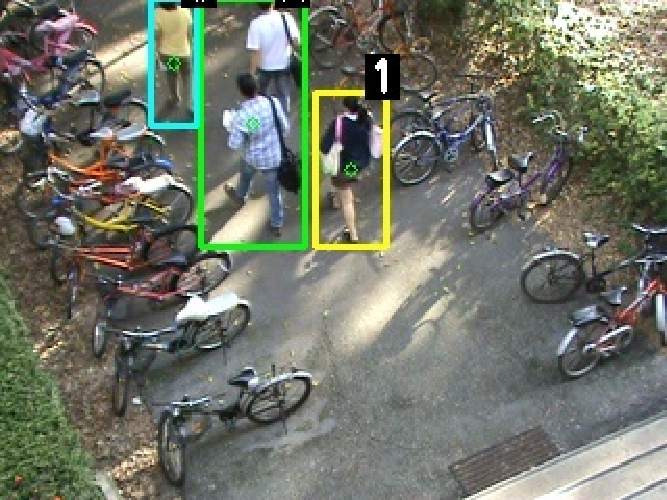
\includegraphics[scale=0.17]{figures/complex-tracking-result-0160} 
            \\
            \small Frame 125 & 
            \small Frame 131 & 
            \small Frame 133 & 
            \small Frame 141 & 
            \small Frame 160
        \end{tabular}
        \caption{Sample blob tracking results for a complex case.}
        \label{fig:complex-tracking-results}
    \end{figure}

\end{frame}

%--------------------------------------------------------------------

\begin{frame}
    \frametitle{Blob-Based Motion Analysis}
    \framesubtitle{Discussion}

    We develop an appearance-based method for blob tracking 
    that uses the forward-backward overlap technique and the 
    color coherence vector (CCV) for occlusion handling.

    \medskip

    Limitations: 
    \begin{itemize}
        \item Our blob tracking method is not robust for complex events 
            involving multiple people.
        \item It also does not allow evolution of the learned bootstrap 
            model over time.
        \item Due to noise, fragmented blobs may affect the results. An 
            effective method to handle blob fragmentation would be 
            recommended.
    \end{itemize}

\end{frame}

